% Toy paper for the AI for Research seminar.
%
% Illustrative only. This skeleton is meant to be filled in by an AI agent
% working from the Stack Overflow Annual Developer Survey data.
% See ../README.md for the workflow.

\documentclass[11pt]{article}

\usepackage[a4paper, margin=2.5cm]{geometry}
\usepackage{graphicx}
\usepackage{booktabs}
\usepackage{hyperref}
\usepackage{natbib}
\usepackage{authblk}

\title{AI-tool adoption and self-reported job satisfaction among professional
software developers: a descriptive analysis of the Stack Overflow Annual
Developer Survey}

\author[1]{Author One}
\author[1]{Author Two}
\affil[1]{Universidade Cat\'olica Portuguesa}

\date{\today}

\begin{document}
\maketitle

\begin{abstract}
We use the 2025 Stack Overflow Annual Developer Survey to describe the
relationship between professional developers' reported adoption of AI coding
tools and their reported job satisfaction, controlling for years of
professional experience and primary developer role. In a complete-case sample
of 24,354 respondents, reported AI-tool adoption is associated with a 0.151-point
higher job-satisfaction score on a 0--10 scale (standard error 0.033,
$p<0.001$). The association is statistically precise but small. The analysis is descriptive: the
survey is observational, selection into the survey is not random, and
both AI-tool adoption and satisfaction are self-reported. We discuss the
limits this design imposes on causal interpretation. This paper is a
teaching artefact produced for a seminar on AI for research; it is not
intended for publication.
\end{abstract}

\section{Introduction}
AI-enabled tools have quickly become part of many software developers' work.
Their adoption may coincide with changes in the experience of work: automation
could remove repetitive tasks, while unreliable output or pressure to adopt new
tools could create frustration. This paper asks a deliberately narrow question:
among professional developers responding to the 2025 Stack Overflow Annual
Developer Survey, is reported AI-tool adoption associated with reported job
satisfaction?

The available data cannot establish whether AI tools change satisfaction.
Adoption is not randomly assigned, and the survey observes respondents at only
one point in time. We therefore estimate a descriptive conditional association,
not a causal effect. The contribution is a transparent worked example for
teaching an end-to-end research workflow: define variables, construct an
analysis sample, run a reproducible regression, inspect figures, and report the
limitations alongside the estimate.

\section{Data}
The data are from the 2025 Stack Overflow Annual Developer Survey
\citep{stackoverflow2025survey}. The downloaded file contains 49,191 responses
and 172 variables. Stack Overflow recruits respondents openly rather than by
probability sampling, so the respondents should not be interpreted as a
representative sample of all software developers. The data are released under
the Open Database License 1.0 and Database Contents License 1.0.

We retain the 37,467 respondents whose main branch identifies them as
professional developers. Job satisfaction is the survey's numeric
\texttt{JobSat} response, measured from 0 to 10. We classify respondents as AI
tool adopters when \texttt{AISelect} reports daily, weekly, or monthly/infrequent
use; the two ``No'' responses form the non-adopter group. Professional
experience is numeric \texttt{WorkExp}. Because \texttt{DevType} can list
multiple roles, we use its first listed role as the primary role. Complete-case
filtering and the exclusion of missing or uncodable AI responses leave 24,354
observations.

\section{Method}
We estimate ordinary least squares regressions of job satisfaction on an
indicator for reported AI-tool adoption, years of professional work experience,
and fixed effects for primary developer role. The model includes 31 role
indicators; ``Developer, full-stack,'' the most common role in the analysis
sample, is the omitted category. We report conventional OLS standard errors.

The coefficient on AI-tool adoption compares adopters and non-adopters with the
same recorded years of experience and primary role. This adjustment addresses
only those measured differences. It does not make adoption exogenous and should
not be read as the effect of using AI tools.

\section{Results}
Table~\ref{tab:results} reports the central descriptive and regression results.
Among the 19,680 reported adopters, mean job satisfaction is 7.236; among the
4,674 non-adopters, it is 7.132. Both groups have a median of 8. Figure~\ref{fig:sat-by-ai}
shows that the raw difference in means is modest.

After adjustment for experience and primary-role fixed effects, the adoption
coefficient is 0.151 satisfaction points (standard error 0.033, $t=4.63$,
$p<0.001$). The model $R^2$ is 0.021. Thus, reported adoption has a positive
cross-sectional association with satisfaction, but the estimated difference is
only about 1.5 percent of the full 0--10 response scale and the model explains
little of the individual variation in satisfaction. Respondents in the analysis
sample report a mean of 13.6 years and a median of 11 years of professional
experience; Figure~\ref{fig:years} shows its right-skewed distribution.

\begin{table}[htbp]
  \centering
  \caption{Job satisfaction and reported AI-tool adoption}
  \label{tab:results}
  \begin{tabular}{lrrr}
    \toprule
    Group or estimate & $N$ & Mean & Median \\
    \midrule
    AI tools not used & 4,674 & 7.132 & 8.00 \\
    AI tools used & 19,680 & 7.236 & 8.00 \\
    \midrule
    \multicolumn{4}{l}{OLS adoption coefficient: 0.151 (SE 0.033; $p<0.001$)} \\
    \multicolumn{4}{l}{Model $N=24,354$; $R^2=0.021$; experience control and role fixed effects included.} \\
    \bottomrule
  \end{tabular}
\end{table}

\begin{figure}[htbp]
  \centering
  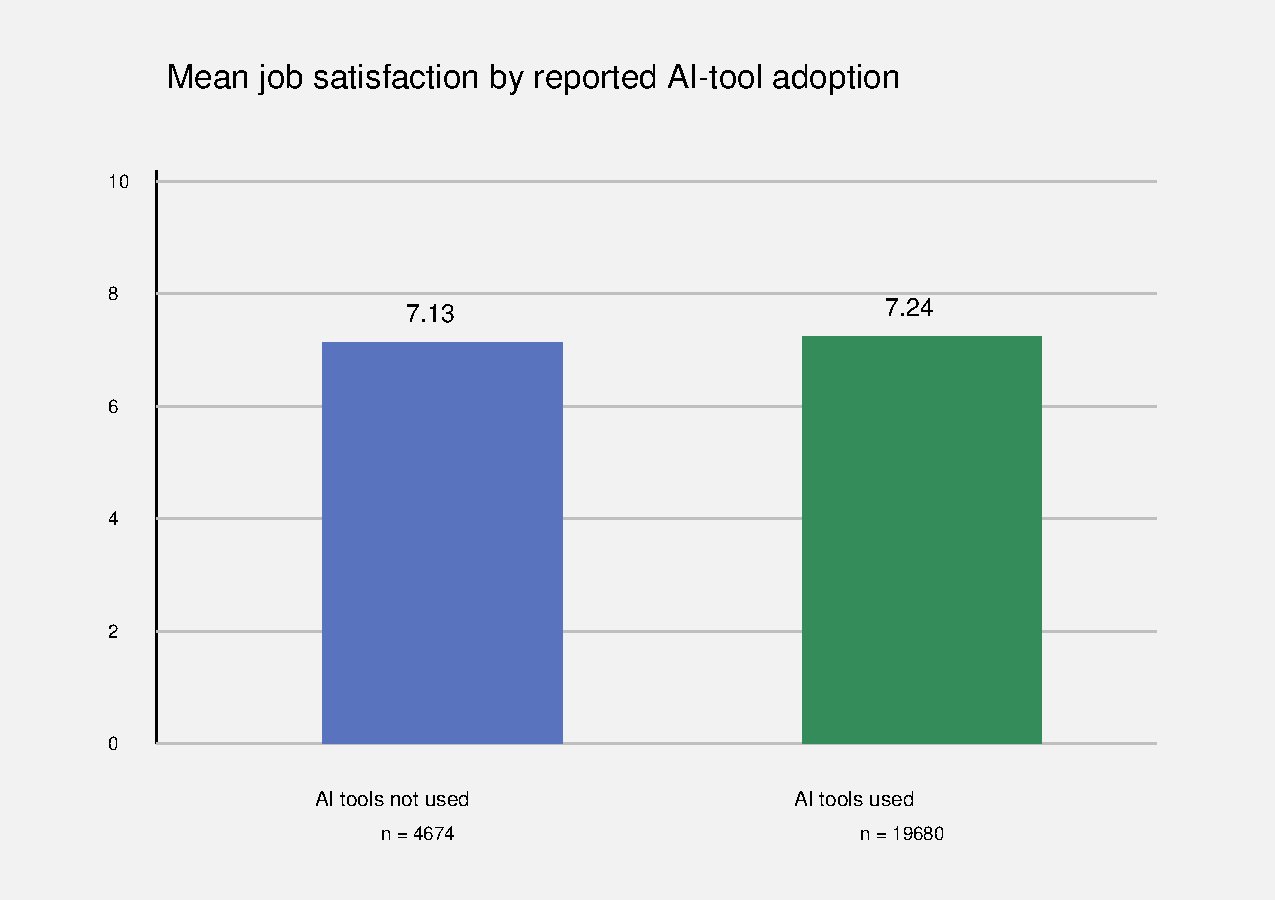
\includegraphics[width=0.8\linewidth]{figures/fig1_satisfaction_by_ai_use.pdf}
  \caption{Self-reported job satisfaction by reported AI-tool use, analysis
  sample.}
  \label{fig:sat-by-ai}
\end{figure}

\begin{figure}[htbp]
  \centering
  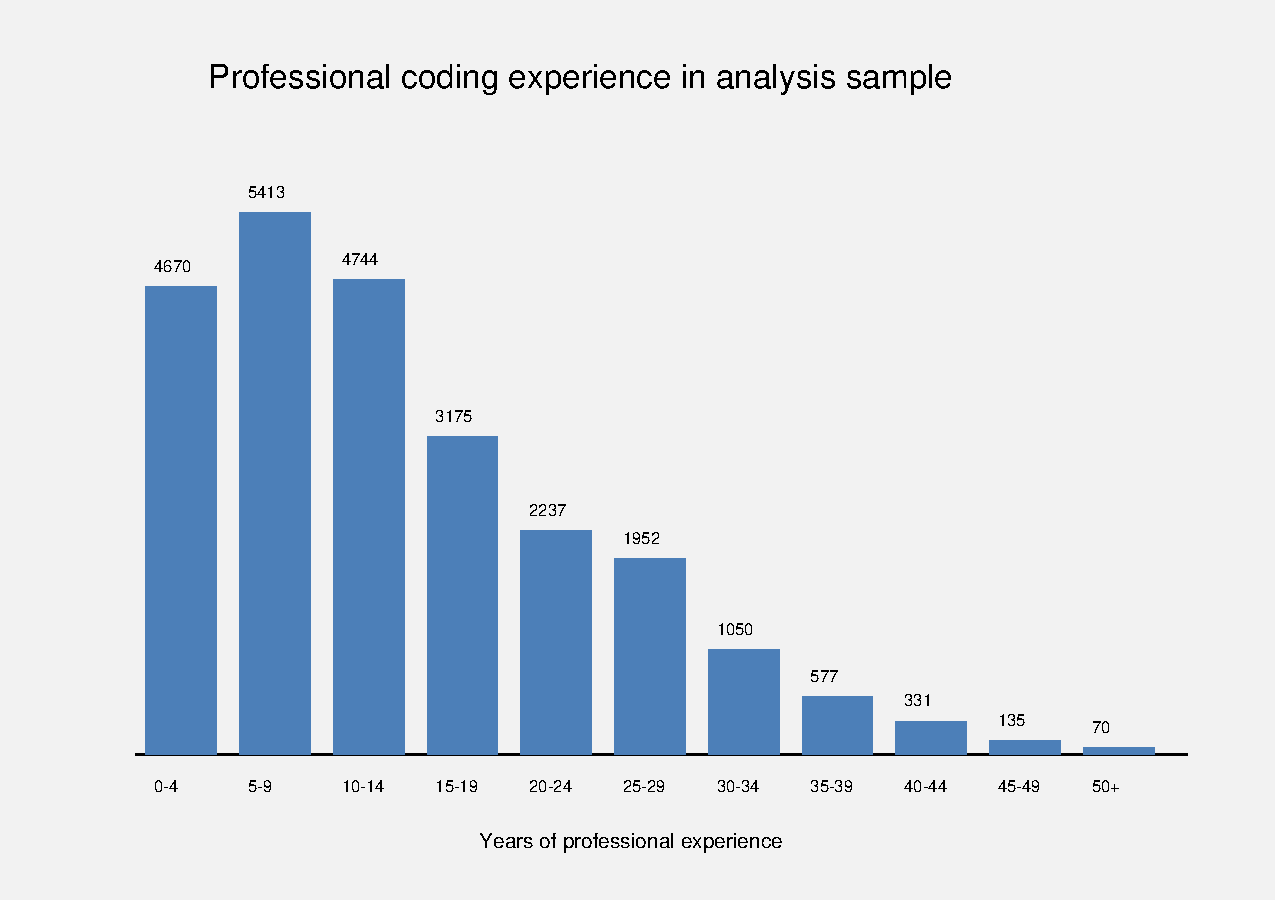
\includegraphics[width=0.8\linewidth]{figures/fig2_years_experience.pdf}
  \caption{Distribution of years of professional coding experience in the
  analysis sample.}
  \label{fig:years}
\end{figure}

\section{Limitations}
The headline limitation is that the estimate is not causal. Selection into the
Stack Overflow survey is not random: developers who encounter the survey and
choose to complete it may differ systematically from other developers. The
sample therefore cannot support population-wide prevalence claims without
strong additional assumptions.

Both central variables are self-reported. Respondents may interpret AI-tool use
differently or misreport its frequency, and a single satisfaction score is an
imperfect measure of work experience. The survey contains no instrument or
other source of plausibly exogenous variation in adoption. Its cross-sectional
design also prevents us from establishing whether adoption preceded
satisfaction.

Finally, the regression controls only for experience and primary role. Omitted
factors such as team culture, employer policy, job quality, developer ability,
pay, and enthusiasm for new technology may influence both adoption and
satisfaction. Any of them could generate or mask the small observed association.
The complete-case restriction and our reduction of multi-role responses to the
first listed role add further scope for selection and measurement error.

\section{Conclusion}
Professional developers who report using AI tools also report slightly higher
job satisfaction in this survey. The adjusted difference is 0.151 points on a
0--10 scale. We document an association, not evidence that AI-tool adoption
causes greater satisfaction; the design cannot distinguish that explanation
from selection, reverse ordering, or omitted variables.

This paper is a teaching artefact rather than a publishable empirical study. Its
purpose is to demonstrate a reproducible path from a public dataset to an
auditable analysis, figures, and a compiled paper while keeping statistical and
substantive uncertainty visible.

\bibliographystyle{plainnat}
\bibliography{refs}

\end{document}
